% !TEX encoding = UTF-8 Unicode
\documentclass[
11pt,
master, % тип документа
subf, % подключить и настроить пакет subfig для вложенной нумерации рисунков
href, % подключить и настроить пакет hyperref
colorlinks=true, % цветные гиперссылки
times, % шрифт Times как основной
%fixint=false % отключить прямые знаки интегралов
]{disser}
\usepackage[left=25mm, top=20mm, right=10mm, bottom=20mm]{geometry}
\usepackage[T2A]{fontenc}
\usepackage[utf8]{inputenc}
\usepackage[english,russian]{babel}
\usepackage{amsmath,amssymb,cmap} % cmap для кодировки шрифтов в pdf
\usepackage{pdfpages} % вставляем pdf файлы
\usepackage{indentfirst} % отделять первую строку раздела абзацным отступом
\usepackage{titletoc} % убираем отступ перед "Оглавление"
\usepackage{graphicx}
\usepackage{setspace}
\usepackage{verbatim} % для оформления кода
\usepackage{pdfsync} % установка соответствия документ - код
\graphicspath{{./Img/}}

\setlength\parindent{5ex} % абзацный отступ равный пяти строчным буквам основного шрифта
\pagestyle{plain} % включаем нумерацию
\setcounter{tocdepth}{2} % включать подсекции в оглавление
\linespread{1.3} % полуторный интервал


% Номера страниц снизу и по центру
\pagestyle{footcenter}
\chapterpagestyle{footcenter}

\begin{document}

\pagestyle{empty}
\begin{center}

\noindent  Федеральное государственное бюджетное образовательное учреждение\\
высшего профессионального образования\\

Московский государственный технический университет им. Н.Э. Баумана \\
Факультет <<Фундаментальные науки>>\bigskip\\

\vfill

Лабораторная работа №8\\
по курсу «Вычислительная физика»\\
Тема: «Одношаговые численные методы решения задачи Коши»\\
\textbf{Вариант 6}\\


\vfill
\vfill
\begin{flushright}
\begin{tabular}{ll}
Выполнили: & студенты группы ФН4-72Б     \\
           & Хижик А.И., Мистрюкова Л.А.  \\
Проверил:  & доцент, к.физ.-мат.н.       \\
           & Хасаншин Р.Х.
\end{tabular}
\end{flushright}
\vfill
\begin{center}
Москва, $2019$
\end{center}

\end{center}
\pagebreak


\pagestyle{plain}
\tableofcontents

\section{Теоретическая часть}
\subsection{Введение}
Одношаговым методом численного решения дифференциального уравнения (ДУ) называют метод, при использовании которого для получения решения в каждой новой узловой точке достаточно иметь значение сеточной функции лишь в предыдущем узле.

Суть разностного метода решения обыкновенных дифференциальных уравнений (ОДУ) заключается в следующем. Область непрерывного изменения аргумента заменяют дискретным множеством точек, называемых узлами. Совокупность этих узлов составляет разностную сетку. Искомую функцию непрерывного аргумента заменяют функцией дискретного аргумента на заданной сетке, которую называют сеточной функцией. Путём аппроксимации производных конечно-разностными соотношениями исходное дифференциальное уравнение заменяют разностным уравнением относительно сеточной функции. Такую замену ДУ разностным называют его аппроксимацией на сетке (или разностной аппроксимацией).

Любая дифференциальная задача может быть представлена в следующем виде:
\begin{equation}\label{eq1}
  L[y] = F(x),\;\; x\in G,
\end{equation}
\begin{equation}\label{eq2}
  l[y] = \Phi(x),\;\; x\in \Gamma.
\end{equation}
где $L, l$ -- линейные дифференциальные операторы, $F(x)$ -- заданная функция, $G$ -- область решения задачи, $\Gamma$ -- область, в которой заданы дополнительные условия.

Введем сетку $g_h$ -- конечное множество точек, принадлежащих области $G$, плотность распределения которых характеризуется параметром $h$ -- шагом сетки; с помощью формул численного дифференцирования заменим линейные дифференциальные операторы $L$, $l$ на разностные аналоги $L_h$, $l_h$; функцию непрерывного аргумента $y(x)$ заменим сеточной функцией $u_h$, а правую часть уравнений (\ref{eq1}-\ref{eq2}) на сеточные функции $f_h(x)$ и $\varphi_h(x)$ соответственно. В результате получим систему разностных уравнений, называемую разностной схемой (РС):
\begin{equation}\label{eq3}
  L_h[u_h] = f_h(x),\;\; x\in g_h,
\end{equation}
\begin{equation}\label{eq4}
  l_h[u_h] = \varphi_h(x),\;\; x\in \gamma_h.
\end{equation}

\subsubsection{Основные понятия теории разностных схем}

Погрешностью РС (\ref{eq3}-\ref{eq4}) называется величина
\begin{equation}\label{eq5}
  \delta_h(x) = u_h(x) - P_h[y(x)],\;\;x\in g_h,
\end{equation}
где $P_h$ -- оператор проектирования.

Выразив из (\ref{eq5}) функцию $u_h(x)$, подставим ее в (\ref{eq3}-\ref{eq4}):
$$L_h[y_h] + L_h[P_h[y(x)]] = f_h(x),$$
$$l_h[y_h] + l_h[P_h[y(x)]] = \varphi_h(x).$$

Функция $\displaystyle R_h(x) = L_h[\delta_h(x)] = f_h(x) - L_h[P_h[y(x)]]$ называется невязкой ДУ, а $\displaystyle r_h(x) = \varphi_h(x) - l_h[P_h[y(x)]]$ -- невязкой для дополнительных условий.

Характерные значения для невязок и погрешности на сетке: $R = \max_{g_h} R_h$, $r = \max_{\gamma_h} r_h$, $\delta = \max_{g_h} \delta_h$.

Если характерные величины для невязок имеют вид $R = O(h^k)$, $r = O(h^k)$, то говорят, что РС (\ref{eq3}-\ref{eq4}) аппроксимирует исходное ДУ порядком $k$.

РС (\ref{eq3}-\ref{eq4}) аппроксимирует исходную дифференциальную задачу (\ref{eq1}-\ref{eq2}), если $\left\|R_h(x)\right\|_h \rightarrow 0$ и $\left\|r_h(x)\right\|_h \rightarrow 0$ при $h\rightarrow 0$.

РС (\ref{eq3}-\ref{eq4}) сходится к решению дифференциальной задачи (\ref{eq1}-\ref{eq2}), если при $h\rightarrow 0$ и $\|u_h - P_h[y]\|_h = \|\delta_h\|_h \rightarrow 0$.

Для того, чтобы РС была сходящейся, необходимо и достаточно, чтобы она была аппроксимирующей и устойчивой.

\subsubsection{Задача Коши}
Рассмотрим задачу Коши для ДУ
\begin{equation}\label{eq}
  u' = f(x,u),\;\;x > x_0,
\end{equation}
с начальным условием $u(x_0) = u_0$.

\textbf{Теорема Коши}: если правая часть ДУ (\ref{eq}) и ее частная производная $f'_u(x,u)$ определены и непрерывны в некоторой области $G'$ изменения переменных $x$ и $u$, то для
всякой внутренней точки $(x_0, u_0)$ этой области данное уравнение
имеет единственное решение, принимающее заданное значение $u_0$ при $x = x_0$.

Методы решения дифференциальной задачи (\ref{eq}) распространяются и на случай систем ДУ, а к ним, в свою очередь, можно привести также уравнения высших порядков.

\subsection{Метод Эйлера}
Метод Эйлера является простейшим численным методом решения задачи Коши для ДУ. Рассмотрим дифференциальную задачу
\begin{equation}\label{eq6}
  y' = f(x,y),\;\;x\in[a,b]
\end{equation}
\begin{equation}\label{eq7}
  y(a) = y_0
\end{equation}

Введем на отрезке $[a,b]$ сетку $g_h = {a = x_0 < x_1 < \ldots < x_N = b}$ с шагом сетки $h_n = x_{n+1} - x_n$. Разложим решение $y(x)$ в окрестности точки $x_n$ в ряд Тейлора:
\begin{equation}\label{eq8}
  y(x_{n+1}) = y(x_n) + h_n y'(x_n) + \frac{1}{2!} h^2_n y''(x_n) + \ldots
\end{equation}

Если функция $f(x,u)$ имеет непрерывные частные производные до порядка $s$, то в выражении (\ref{eq8}) можно оставить члены вплоть до $O(h_n^{s+1})$, тогда, например, первую и вторую производные соответственно можно представить в виде
$$y'(x_n) = f(x_n, y(x_n))$$
$$y''(x_n) = \frac{dy'}{dx}(x_n) = f'_y(x_n, y(x_n))y'(x_n) + f'_x(x_n) = f\frac{\partial f}{\partial y}(x_n) + \frac{\partial f}{\partial x}(x_n)$$

Использование выражения (\ref{eq8}) с большим числом членов имеет следующие основные недостатки:
\begin{enumerate}
  \item С увеличением порядка производных выражения для них усложняются;
  \item Если функция $f$ известна лишь приближено или задана в виде таблицы, ее производные вычисляются с большой погрешностью.
\end{enumerate}

Поэтому в ряде оставляют только два первых члена. При такой замене вместо точного решения $y(x_{n+1})$ в узловых точках получают его приближённое значение $u_{n+1}$:
\begin{equation}\label{eq9}
  u_{n+1} = u_n + h_n f(x_n,u_n),\;\;n=\overline{0,N-1}.
\end{equation}

Поскольку значение $u_0 = y_0$ известно из начальных условий (\ref{eq7}), то, используя формулу (\ref{eq9}), последовательно находим $u_1,\ldots,u_N$ -- приближённое значение дифференциальной задачи (\ref{eq6}-\ref{eq7}) в узловых точках. Формулу (\ref{eq9}) для равномерной сетки ($h_n = h = const$),
\begin{equation}\label{eq10}
  u_{n+1} = u_n + hf(x_n,u_n),
\end{equation}
называют методом Эйлера (методом ломанных).

\subsubsection{Погрешность метода}
Погрешность при использовании метода обусловлена тем, что приращение значения функции при переходе от точки $x_n$, $n = \overline{0,N-1}$ к точке $x_{n+1}$ заменяется приращением ординаты касательной к соответствующей интегральной кривой.

Погрешность $\delta_n$ в точке $x_n$ равна разности точного решения дифференциальной задачи (\ref{eq6}-\ref{eq7}) $y(x_n)$ и значения сеточной функции $u_n$:
\begin{equation}\label{eq11}
  \delta_n = y(x_n) - u_n \rightarrow u_n = y(x_n) - \delta_n,
\end{equation}
\begin{equation}\label{eq12}
  \delta_{n+1} = y(x_{n+1}) - u_{n+1} \rightarrow u_{n+1} = y(x_{n+1}) - \delta_{n+1}.
\end{equation}
Подставим выражения (\ref{eq11}-\ref{eq12}) в формулу (\ref{eq10}):
\begin{equation}\label{eq13}
  y(x_{n+1}) - \delta_{n+1} = y(x_n) - \delta_n + hf(x_n,y(x_n) - \delta_n).
\end{equation}
Разложим функцию $f$ в ряд в окрестности точки $(x_n,y(x_n))$:
$$f(x_n,y(x_n)-\delta_n) = f(x_n,y(x_n)) - \delta_n \frac{\partial f}{\partial y} + O(\delta_n^2) = f(x_n,y(x_n)) + O(\delta_n).$$
Следовательно,
$$\delta_{n+1} - \delta_n = O(h^2) + h O(\delta_h),$$
где первое слагаемое определяет погрешность аппроксимации производной, а второе -- неточность значения $u_h$.

Для нахождения значения $u_1$ используем начальное значение $u_0 = y_0$, которое задаётся, как правило, точно, т.е. $\delta_0 = 0$. Отсюда $\delta_1 = O(h^2), \delta_2 = \delta_1 + O(h^2) + hO(h^2) = \delta_1 + O(h^2),\ldots, \delta_{n+1} = \delta_n + O(h^2)$, $n = \overline{0,N-1}$. $\delta_n$ называется локальной погрешность. Поскольку $h=\frac{b-a}{N}$, то для погрешности на сетке $\delta_N$ (глобальной погрешности) получим следующее соотношение
$$\delta_N = NO(h^2) = \frac{b-a}{h} O(h^2) = O(h).$$

Таким образом, метод Эйлера имеет первый порядок точности на сетке и второй порядок точности на шаге.

\subsection{Модифицированный метод Эйлера}
Рассмотрим дифференциальное уравнение (\ref{eq6}) в окрестности точки $x = x_n +\frac{h}{2}$, $n = \overline{0,N-1}$, являющейся серединой отрезка $[x_n ,x_{n+1}]$. В левой части дифференциального уравнения (\ref{eq6}) производную заменим центральной разностью
$$y'\left(x_n + \frac{h}{2}\right) \approx \frac{u_{n+1}-u_n}{h},$$
а в правой части уравнения значением функции $f\left(x_n + \frac{h}{2}, y(x_n + \frac{h}{2})\right)$ -- средним арифметическим значением функции в точках $(x_n, u_n)$ и $(x_{n+1}, u_{n+1})$. Тогда
\begin{equation}\label{eq14}
  u_{n+1} = u_n + \frac{h}{2}[f(x_n, u_n) + f(x_{n+1}, u_{n+1})].
\end{equation}
Если искомое решение $u_{n+1}$ входит в правую часть уравнения (\ref{eq14}) и оно не может быть разрешено относительно $u_{n+1}$, то формулу (\ref{eq14}) называют неявной схемой. Для вычисления значения $u_{n+1}$ можно применить один из итерационных методов. Если имеется значение $u_n$, то решение можно построить с использованием двух итераций следующим образом. Считая значение $u_n$ начальным приближением, вычислим первое приближение $\tilde{u}_{n+1}$ к значению $u_{n+1}$ по формуле (\ref{eq10}) метода Эйлера:
\begin{equation}\label{eq15}
  \tilde{u}_{n+1} = u_n + h f(x_n, u_n).
\end{equation}

Вычисленное значение $\tilde{u}_{n+1}$ подставим вместо $u_{n+1}$ в правую часть уравнения (\ref{eq14}) и найдем окончательное значение $u_{n+1}$:
\begin{equation}\label{eq16}
  u_{n+1} = u_n + \frac{h}{2}[f(x_n, u_n) + f(x_{n+1}, \tilde{u}_{n+1})].
\end{equation}

Таким образом, получили следующие соотношения:
\begin{equation}\label{eq17}
  u_{n+1} = u_n + \frac{h}{2}[f(x_n, u_n) + f(x_{n+1}, u_n + h f(x_n, u_n))],\;\;n=\overline{0,N-1}.
\end{equation}

Рекуррентные соотношения (\ref{eq16}) описывают модифицированный метод Эйлера.

При замене производной в левой части уравнения (\ref{eq6}) центральной разностью допускается погрешность порядка $O(h^2)$. Покажем, что погрешность такого же порядка допускается при замене правой части уравнения (\ref{eq6}) в точке $x = x_n + \frac{h}{2}$ средним арифметическим значением функции $f(x,y(x))$ в точках $(x_n, u_n)$ и $(x_{n+1}, u_{n+1})$. Действительно, разложим $f(x, y(x))$ в окрестности точки $\left(x_n + \frac{h}{2}, y\left(x_n + \frac{h}{2}\right)\right)$:
\begin{align*}
	\frac{1}{2}[f(x_n, u_n) + f(x_{n+1}, u_{n+1})] &= \frac{1}{2}\big[f\left[x_n + \frac{h}{2}, y\left(x_n + \frac{h}{2}\right)\right] - \frac{h}{2}\left(\frac{\partial f}{\partial x} + \frac{\partial f}{\partial y}y'\right) + O(h^2) +\\
	& + f\left[x_n + \frac{h}{2}, y\left(x_n + \frac{h}{2}\right)\right] + \frac{h}{2}\left(\frac{\partial f}{\partial x} + \frac{\partial f}{\partial y}y'\right) + O(h^2)\big] = \\
	& = f\left[x_n + \frac{h}{2}, y\left(x_n + \frac{h}{2}\right)\right] + O(h^2)
\end{align*}

Таким образом, погрешность вычислений составляет $hO(h^2) = O(h^3)$. Этот порядок погрешности сохраняется и при использовании двух итераций, поскольку
$$f(x_{n+1}, \tilde{u}_{n+1}) = f(x_{n+1}, u_{n+1}) + \frac{\partial f}{\partial y}(\tilde{u}_{n+1} - u_{n+1}) + O(h^2) = f(x_{n+1}, u_{n+1}) + O(h^2).$$
Следовательно, локальная погрешность имеет порядок $O(h^3)$, а глобальная -- $O(h^2)$, т.е. модифицированный метод Эйлера имеет второй порядок точности.

\subsection{Усовершенствованный метод Эйлера}
Также как и в случае модифицированного метода Эйлера, рассмотрим ДУ (\ref{eq6}) в окрестностях точек $x = x_n + \frac{h}{2}$, $n = \overline{0,N-1}$. Левую часть ДУ заменим центральной разностью, а правую оставим без изменений:
\begin{equation}\label{eq18}
  \frac{u_{n+1}-u_n}{h} = f\left(x_n + \frac{h}{2}, y\left(x_n + \frac{h}{2}\right)\right).
\end{equation}

Приближённое значение функции $y(x)$ в точке $\left(x_n + \frac{h}{2}\right)$ вычислим с помощью метода Эйлера:
\begin{equation}\label{eq19}
  \tilde{u}_{n+1} = u_n + \frac{h}{2} f(x_n, u_n).
\end{equation}

Выразим $u_{n+1}$ из (\ref{eq18}), заменив $y\left(x_n + \frac{h}{2}\right)$ его приближением $\tilde{u}_{n+1}$ по формуле (\ref{eq10}):
\begin{equation}\label{eq201}
  u_{n+1} = u_n + hf\left(x_n + \frac{h}{2}, \tilde{u}_{n+1}\right).
\end{equation}

Алгоритм решения дифференциальной задачи (\ref{eq6}-\ref{eq7}) по формулам (\ref{eq19}-\ref{eq201}) называют усовершенствованным методом Эйлера.

\subsection{Метод Эйлера-Кромера}
Метод Эйлера-Кромера является улучшенной модификацией метода Эйлера.

Рассмотрим классическое уравнение движение материальной точки
\begin{equation}\label{eq20}
  \ddot{x} = f(x,\dot{x},t),\;\;t>t_0,
\end{equation}
с начальными условиями $x(t_0) = x_0$, $\dot{x}(t_0) = \upsilon_0$.

Уравнение (\ref{eq20}) можно представить в виде системы
$\left\{
  \begin{array}{ll}
    \dot{\upsilon}(t) = f(x,\upsilon,t),\\
    \dot{x}(t) = \upsilon.
  \end{array}
\right.$

Введем сетку $g_\tau = \{t_n\}$, $t_n = n\tau$, $n = 0,1,2,\ldots$, где $\tau$ - шаг сетки.

Алгоритм решения методом Эйлера-Кромера:
$$\upsilon_{n+1} = \upsilon_n + \tau f(x_n, \upsilon_n, t_n),$$
$$x_{n+1} = x_n + \tau \upsilon_{n+1}.$$

Алгоритм решения методом Эйлера:
$$\upsilon_{n+1} = \upsilon_n + \tau f(x_n, \upsilon_n, t_n),$$
$$x_{n+1} = x_n + \tau \upsilon_n.$$

Метод Эйлера-Кромера, несмотря на первый порядок точности, в случае решения уравнения колебаний вида (\ref{eq20}) значительно повышает реальную точность по сравнению с явным методом Эйлера, особенно при больших значениях $t$. В методе Эйлера-Кромера повышенная точность обеспечивается тем, что при вычислении нового значения координаты $x_{n+1}$ используется значение скорости материальной точки $\upsilon_{n+1}$ в новой узловой точке.

\subsection{Метод Рунге-Кутта четвёртого порядка}
Основная идея методов Рунге-Кутта повышенной точности заключается в построении специального алгоритма решения задач Коши для ОДУ, такого, чтобы максимально приблизить приращение сеточной функции $\Delta u = u_{n+1} - u_n$ на шаге $n+1$ к приращению точного решения $\Delta y = y(x_{n+1}) - y(x_n)$, которое определяется из ряда Тейлора (\ref{eq8}) в окрестности точки $x_n$ с учётом возможно большего числа членов ряда. При этом, чтобы избежать громоздких выражений, приводящих к увеличению погрешности метода Рунге-Кутта, вторые и последующие производные определяют не дифференцированием, а путём многократного вычисления правой части дифференциального уравнения -- функции $f(x,y)$ в некоторых
промежуточных точках.

Широкое применение для численного решения задач Коши для дифференциальных уравнений получил метод Рунге-Кутта четвёртого порядка. Его алгоритм для решения дифференциальной
задачи (\ref{eq6}-\ref{eq7}) выглядит следующим образом:
\begin{equation}\label{eq21}
  u_{n+1} = u_n + \frac{h}{6}(k_0 + 2k_1 + 2k_2 + k_3),\;\; n = 0,1,\ldots,
\end{equation}
$k_0 = f(x_n, u_n)$, $k_1 = f\left(x_n + \frac{h}{2}, u_n + \frac{hk_0}{2}\right)$, $k_2 = f\left(x_n + \frac{h}{2}, u_n + \frac{hk_1}{2}\right)$, $k_3 = f(x_n + h, u_n + hk_2)$.

Метод Рунге-Кутта требует на каждом шаге четырёхкратного вычисления правой части $f(x,y(x))$ ДУ (\ref{eq6}). Глобальная погрешность этого метода имеет порядок $O(h^4)$, а локальная погрешность -- $O(h^5)$.

Таким образом, метод Рунге-Кутта в отличие от метода Эйлера и его модификаций связан с большим объёмом вычислений, однако это окупается повышенной точностью, что даёт возможность проводить счёт с большим шагом.


\newpage
\section{Постановка задачи}
\begin{itemize}
  \item Решить задачу Коши для дифференциального уравнения $u' = (2-u)\tan(x)$, $x\in [0,1]$ с начальным условием $u(0) = -1$, используя метод Эйлера, модифицированный метод Эйлера, усовершенствованный метод Эйлера и метод Рунге-Кутта четвёртого порядка.
  \item Решить методом Эйлера и методом Эйлера-Кромера задачу об апериодическом колебательном движении:
    $$\ddot{x} + 2\lambda \dot{x} + \omega_0^2 x = 0,\;\;0<t<T,\;\;\lambda > \omega_0,\;\; T = \frac{3}{\lambda},$$
    $$x(0) = 0,\;\; \dot{x}(0) = \upsilon_0.$$

    Сравнить численное решение с аналитическим
    $$x(t) = \frac{\upsilon_0}{\theta}\exp(-\lambda t)\sinh(t\theta),\;\;\theta = \sqrt{\lambda^2 - \omega_0^2},$$
    где $\omega_0 = \frac{1}{2}$, $\lambda = 1$, $\upsilon_0 = 1$.

    Построить графики точного и численного решений, а также графики погрешности $\delta_n = x(t_n) - x_n$.
  \item Решить методом Эйлера и методом Эйлера-Кромера задачу о свободных затухающих колебаниях:
    $$\ddot{x} + 2\lambda \dot{x} + \omega_0^2 x = 0,\;\;0<t<2T,\;\;\lambda < \omega_0,\;\; T = \frac{2\pi}{\omega},$$
  $$\omega = \sqrt{\omega_0^2 - \lambda^2},\;\;\omega_0 > \lambda,\;\;x(0) = 0,\;\; \dot{x}(0) = \upsilon_0.$$

  Сравнить численное решение с аналитическим
  $$x(t) = \frac{\upsilon_0}{\omega}\exp(-\lambda t)\sin(\omega t),$$
  где $\omega_0 = 1$, $\lambda = 0.1$, $\upsilon_0 = 1$.

  Построить графики точного и численного решений, а также графики погрешности $\delta_n = x(t_n) - x_n$.
\end{itemize}

\newpage
\section{Программа}
\subsubsection{Задание А}
{\footnotesize
\begin{verbatim}
#include <iostream>
#include <fstream>

using std::cout;
using std::cin;
using std::endl;
using std::ofstream;

double a = 0, b = 1, y_zero = -1;
int N = 1000;
double h = (b-a) / N;
double fun(double x, double y);
double fun_ex(double x);
void Euler_Method(double* x, double* y, double* delta, int i);
void Modified_Euler_Method(double* x, double* y, double* delta, int i);
void Improved_Euler_Method(double* x, double* y, double* delta, int i);
void RungeKutta(double* x, double* y, double* delta, int i);

int main() {
    double *y = new double[N+1];
    double *x = new double[N+1];
    double *delta = new double[N+1];
    y[0] = y_zero;
    x[N] = b;
    int i;
    for(i=0; i<=N; i++){
        x[i] = a + i*h;
    }

    cout << "EM" << endl;
    Euler_Method(x, y, delta, i);

    cout << endl << "MEM" << endl;
    Modified_Euler_Method(x, y, delta, i);

    cout << endl << "IEM" << endl;
    Improved_Euler_Method(x, y, delta, i);

    cout << endl << "R-K" << endl;
    RungeKutta(x, y, delta, i);
    return 0;
}
void Euler_Method(double* x, double* y, double* delta, int i){
    ofstream fout("Euler_Method");
    for(i=0; i<=N; i++){
        y[i+1] = y[i] + h*fun(x[i],y[i]);
        delta[i] = fun_ex(x[i]) - y[i];
        cout << i << "\t" << x[i] << "\t" << y[i] << "\t" << delta[i] << endl;
        fout << i << "\t" << x[i] << "\t" << y[i] << "\t" << delta[i] << endl;
    }
    fout.close();
}
void Modified_Euler_Method(double* x, double* y, double* delta, int i){
    ofstream fout("Modified_Euler_Method");
    for(i=0; i<=N; i++){
        y[i+1] = y[i] + h*(fun(x[i],y[i]) + fun(x[i+1],y[i] + h*fun(x[i],y[i]))) / 2;
        delta[i] = fun_ex(x[i]) - y[i];
        cout << i << "\t" << x[i] << "\t" << y[i] << "\t" << delta[i] << endl;
        fout << i << "\t" << x[i] << "\t" << y[i] << "\t" << delta[i] << endl;
    }
    fout.close();
}
void Improved_Euler_Method(double* x, double* y, double* delta, int i){
    ofstream fout("Improved_Euler_Method");
    for(i=0; i<=N; i++){
        y[i+1] = y[i] + h*fun(x[i] + h / 2, y[i] + h * fun(x[i], y[i]) / 2);
        delta[i] = fun_ex(x[i]) - y[i];
        cout << i << "\t" << x[i] << "\t" << y[i] << "\t" << delta[i] << endl;
        fout << i << "\t" << x[i] << "\t" << y[i] << "\t" << delta[i] << endl;
    }
    fout.close();
}
void RungeKutta(double* x, double* y, double* delta, int i){
    ofstream fout("RungeKutta");
    double *k0 = new double[N+1];
    double *k1 = new double[N+1];
    double *k2 = new double[N+1];
    double *k3 = new double[N+1];
    for(i=0; i<=N; i++){
        k0[i] = fun(x[i], y[i]);
        k1[i] = fun(x[i] + h / 2, y[i] + h * k0[i] / 2);
        k2[i] = fun(x[i] + h / 2, y[i] + h * k1[i] / 2);
        k3[i] = fun(x[i] + h, y[i] + h * k2[i]);
        y[i+1] = y[i] + h * (k0[i] + 2 * k1[i] + 2 * k2[i] + k3[i]) / 6;
        delta[i] = fun_ex(x[i]) - y[i];
        cout << i << "\t" << x[i] << "\t" << y[i] << "\t" << delta[i] << endl;
        fout << i << "\t" << x[i] << "\t" << y[i] << "\t" << delta[i] << endl;
    }
    fout.close();
}
double fun(double x, double y){
    return (2-y) * tan(x);
}
double fun_ex(double x) {
    return -3 * cos(x) + 2;
}
\end{verbatim}
}

\subsubsection{Задание Б}
{\footnotesize
\begin{verbatim}
#include <iostream>
#include <cmath>
#include <fstream>

using std::cout;
using std::cin;
using std::endl;
using std::ofstream;

double N = 1000;
double lambda = 1, omega_zero = 1. / 2, upsilon_zero = 1, x_zero = 0;
double T = 3 / lambda;
double tau = T / N;
double theta = sqrt(pow(lambda, 2) - pow(omega_zero, 2));

void Euler_Method(double* x, double* v, double* t, double* delta, int i);
void Euler_Kromer(double* x, double* v, double* t, double* delta, int i);
double fun_ex(double t);
double fun(double x, double v);
int main() {
    double *x = new double[N+1];
    double *v = new double[N+1];
    double *t = new double[N+1];
    double *delta = new double[N+1];
    x[0] = x_zero;
    v[0] = upsilon_zero;
    int i;
    for(i=0; i<=N; i++){
        t[i] = i * tau;
    }
    cout << "EM" << endl;
    Euler_Method(x, v, t, delta, i);

    cout << endl << "E-K" << endl;
    Euler_Kromer(x, v, t, delta, i);
    return 0;
}
void Euler_Method(double* x, double* v, double* t, double* delta, int i){
    ofstream fout("Euler_Method");
    for(i=0; i<=N; i++){
        v[i + 1] = v[i] + tau * fun(x[i], v[i]);
        x[i + 1] = x[i] + tau * v[i];
        delta[i] = fun_ex(t[i]) - x[i];
        cout << i << "\t" << t[i] << "\t" << v[i] << "\t" << x[i] << "\t" << delta[i] << endl;
        fout << i << "\t" << t[i] << "\t" << v[i] << "\t" << x[i] << "\t" << delta[i] << endl;
    }
    fout.close();
}
void Euler_Kromer(double* x, double* v, double* t, double* delta, int i){
    ofstream fout("Euler_Kromer");
    for(i=0; i<=N; i++){
        v[i + 1] = v[i] + tau * fun(x[i], v[i]);
        x[i + 1] = x[i] + tau * v[i + 1];
        delta[i] = fun_ex(t[i]) - x[i];
        cout << i << "\t" << t[i] << "\t" << v[i] << "\t" << x[i] << "\t" << delta[i] << endl;
        fout << i << "\t" << t[i] << "\t" << v[i] << "\t" << x[i] << "\t" << delta[i] << endl;
    }
    fout.close();
}
double fun(double x, double v){
    return -2 * lambda * v - pow(omega_zero, 2) * x ;
}
double fun_ex(double t){
    return upsilon_zero * exp(- t * lambda ) * sinh(t * theta) / theta;
}
\end{verbatim}
}

\newpage
\section{Результаты вычислений}
\subsection{Задание А}
\begin{figure}[h]
\begin{minipage}[h]{1\linewidth}
\center{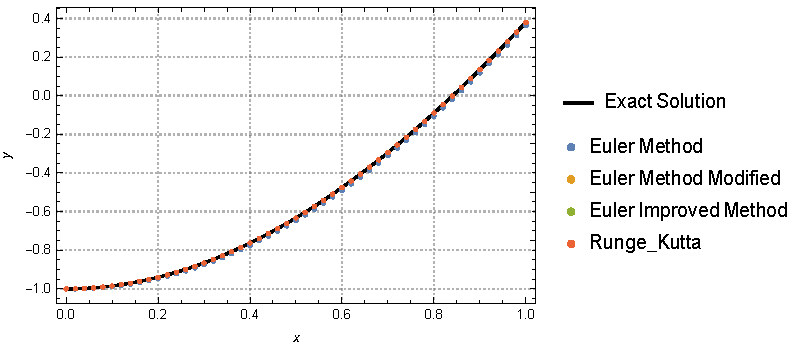
\includegraphics[width=0.8\linewidth]{plEX_50.pdf}} a) \\
\end{minipage}
\vfill
\begin{minipage}[h]{1\linewidth}
\center{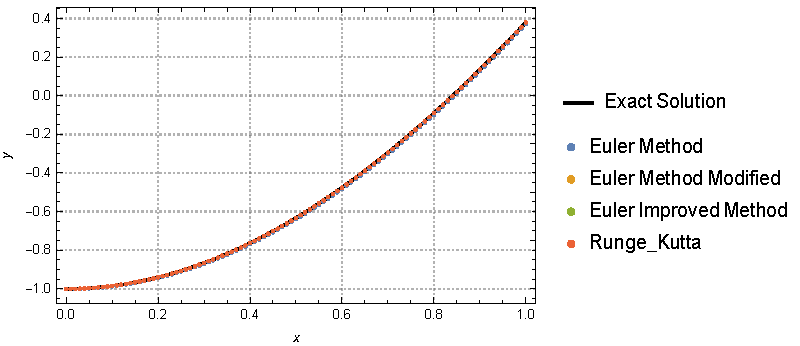
\includegraphics[width=0.8\linewidth]{plEX_100.pdf}} b) \\
\end{minipage}
\vfill
\begin{minipage}[h]{1\linewidth}
\center{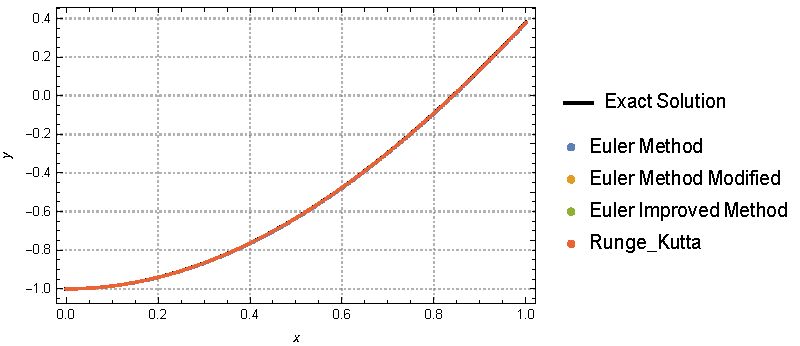
\includegraphics[width=0.8\linewidth]{plEX_250.pdf}} c) \\
\end{minipage}
\caption{Результаты точного и численного решений задачи Коши для ДУ $y' = (2-y) \tan(x)$, $x\in [0,1]$, $y(0) = -1$ стандартным, модифицированным, усовершенствованным методами Эйлера и методом Рунге-Кутта четвёртого порядка для a) $N = 50$, b) $N = 100$, с) $N = 250$.}
\label{ris:1}
\end{figure}

\newpage
\subsection{Задание Б}
\begin{figure}[h]
\begin{minipage}[h]{1\linewidth}
\center{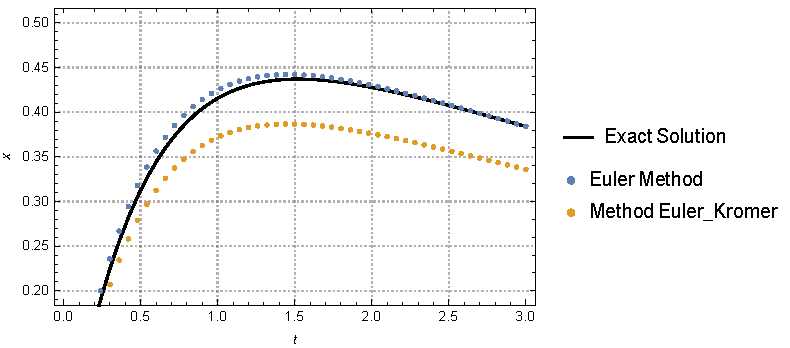
\includegraphics[width=0.78\linewidth]{plVIS_50.pdf}} a) \\
\end{minipage}
\vfill
\begin{minipage}[h]{1\linewidth}
\center{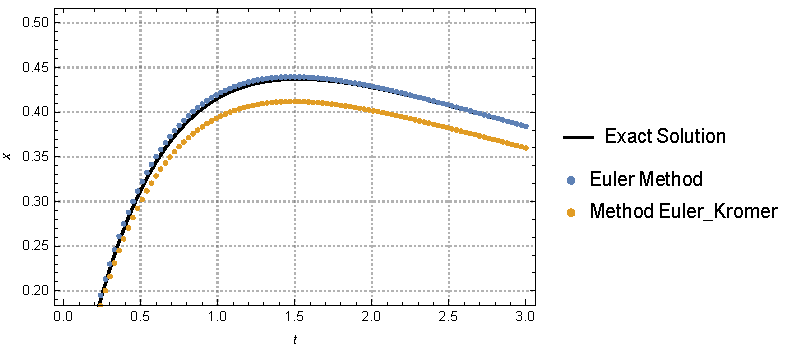
\includegraphics[width=0.78\linewidth]{plVIS_100.pdf}} b) \\
\end{minipage}
\vfill
\begin{minipage}[h]{1\linewidth}
\center{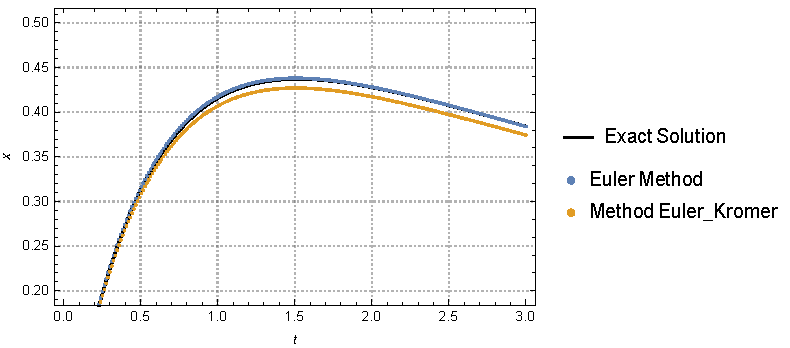
\includegraphics[width=0.78\linewidth]{plVIS_250.pdf}} c) \\
\end{minipage}
\caption{Результаты точного и численного решений задачи об апериодическом колебательном движении: $\ddot{x} + 2 \dot{x} + \frac{x}{4} = 0$, $0<t<3$, $x(0) = 0$, $\dot{x}(0) = 1$  методами Эйлера и Эйлера-Кромера для a) $N = 50$, b) $N = 100$, с) $N = 250$.}
\label{ris:2}
\end{figure}

\newpage
\begin{figure}[h!]
\begin{minipage}[h]{1\linewidth}
\center{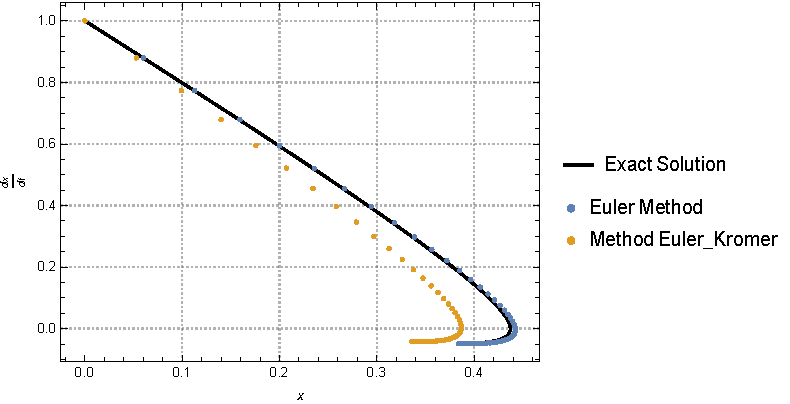
\includegraphics[width=0.7\linewidth]{plF_50.pdf}} a) \\
\end{minipage}
\vfill
\begin{minipage}[h]{1\linewidth}
\center{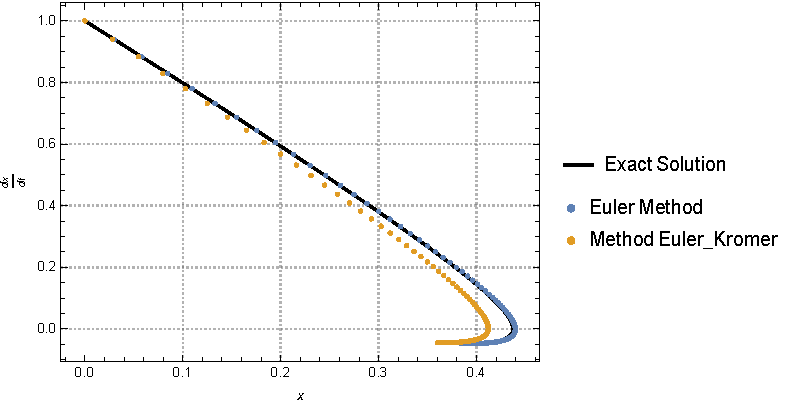
\includegraphics[width=0.7\linewidth]{plF_100.pdf}} b) \\
\end{minipage}
\vfill
\begin{minipage}[h]{1\linewidth}
\center{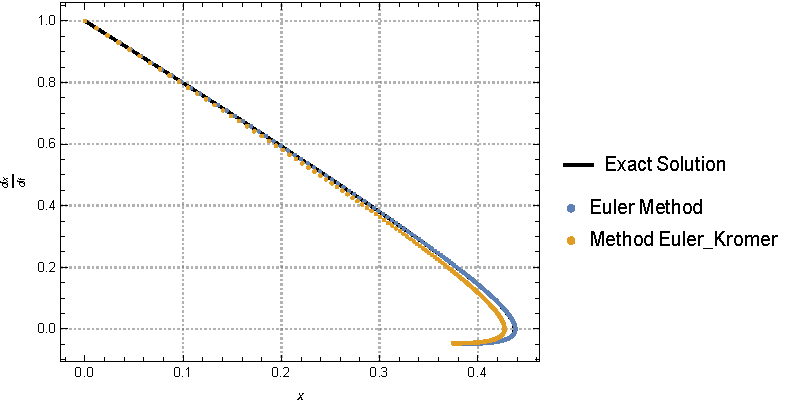
\includegraphics[width=0.7\linewidth]{plF_250.pdf}} c) \\
\end{minipage}
\caption{Фазовые портреты для точного и численного решений при a) $N = 50$, b) $N = 100$, c) $N = 250$.}
\label{ris:3}
\end{figure}

\newpage
\begin{figure}[h]
  \centering
  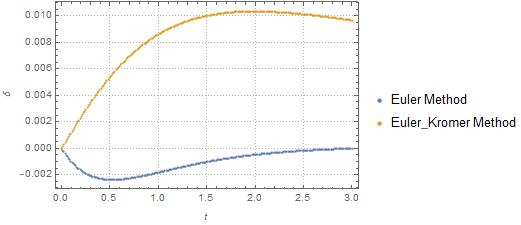
\includegraphics[width=1\linewidth]{plRESer_250}
  \caption{Погрешность вычисления при $N = 250$.}
  \label{ris:4}
\end{figure}

\newpage
\subsection{Задание С}
\begin{figure}[h!]
\begin{minipage}[h]{1\linewidth}
\center{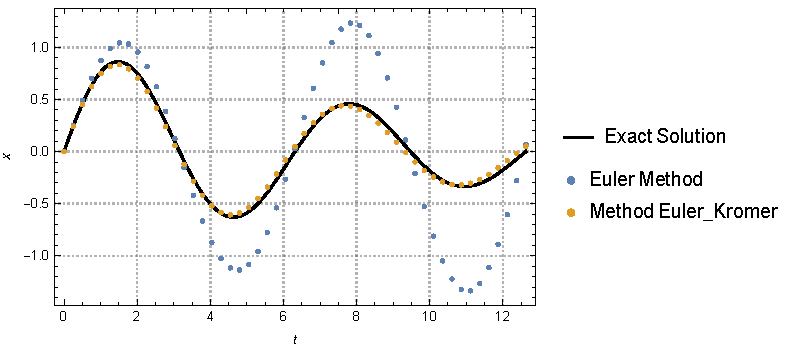
\includegraphics[width=0.78\linewidth]{plVIS1_50.pdf}} a) \\
\end{minipage}
\vfill
\begin{minipage}[h]{1\linewidth}
\center{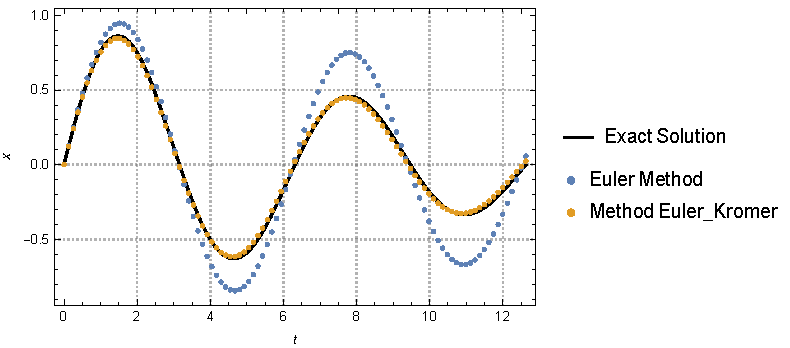
\includegraphics[width=0.78\linewidth]{plVIS1_100.pdf}} b) \\
\end{minipage}
\vfill
\begin{minipage}[h]{1\linewidth}
\center{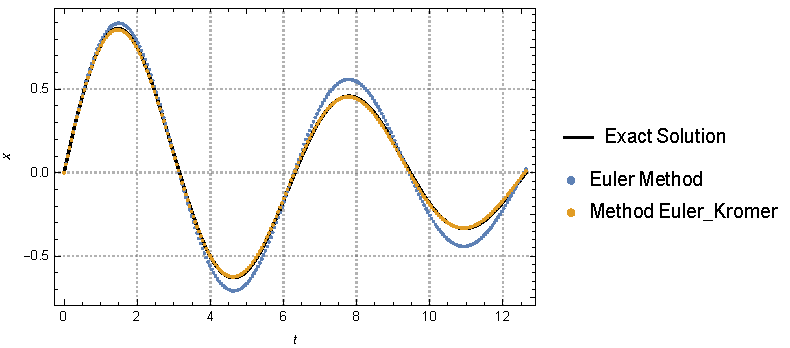
\includegraphics[width=0.78\linewidth]{plVIS1_250.pdf}} c) \\
\end{minipage}
\caption{Результаты точного и численного решений задачи о свободных затухающих колебаниях:\\
 $\ddot{x} + 0.2 \dot{x} + x = 0$, $0<t<\frac{2 \pi}{3\sqrt{11}}$, $x(0) = 0$, $\dot{x}(0) = 1$  методами Эйлера и Эйлера-Кромера для a) $N = 50$,\\
  b) $N = 100$, с) $N = 250$.}
\label{ris:5}
\end{figure}

\newpage
\begin{figure}[h!]
\begin{minipage}[h]{1\linewidth}
\center{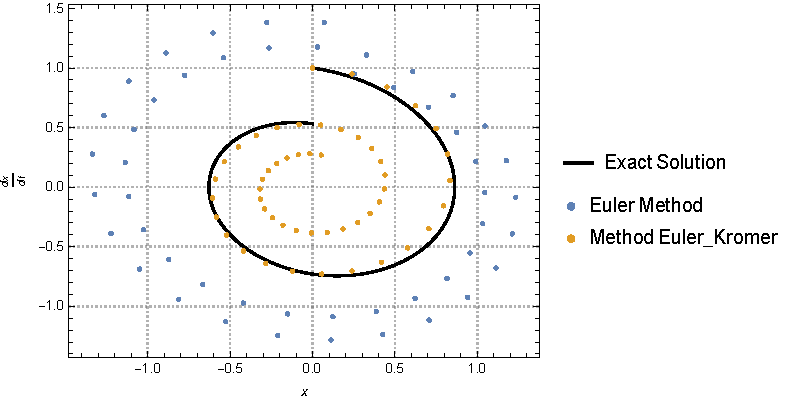
\includegraphics[width=0.7\linewidth]{plF1_50.pdf}} a) \\
\end{minipage}
\vfill
\begin{minipage}[h]{1\linewidth}
\center{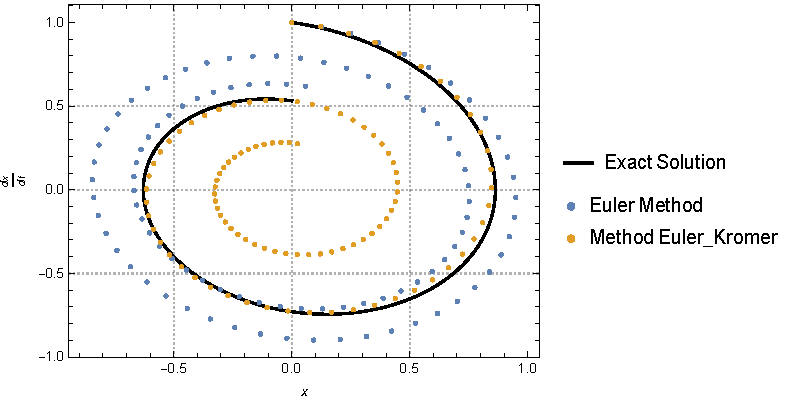
\includegraphics[width=0.7\linewidth]{plF1_100.pdf}} b) \\
\end{minipage}
\vfill
\begin{minipage}[h]{1\linewidth}
\center{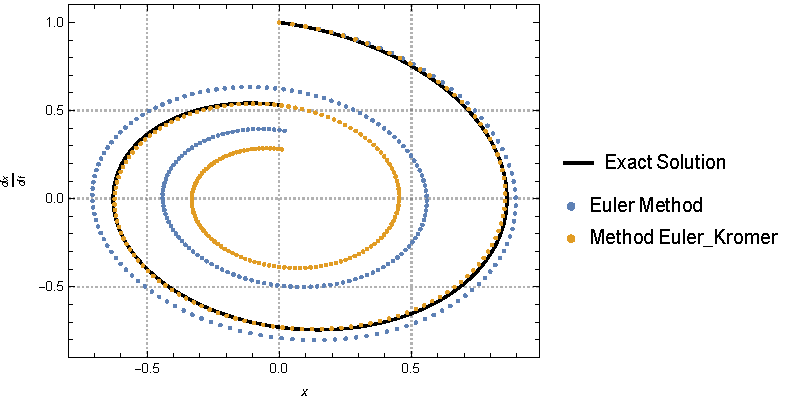
\includegraphics[width=0.7\linewidth]{plF1_250.pdf}} c) \\
\end{minipage}
\caption{Фазовые портреты для точного и численного решений при a) $N = 50$, b) $N = 100$, c) $N = 250$.}
\label{ris:6}
\end{figure}

\newpage
\begin{figure}[h]
  \centering
  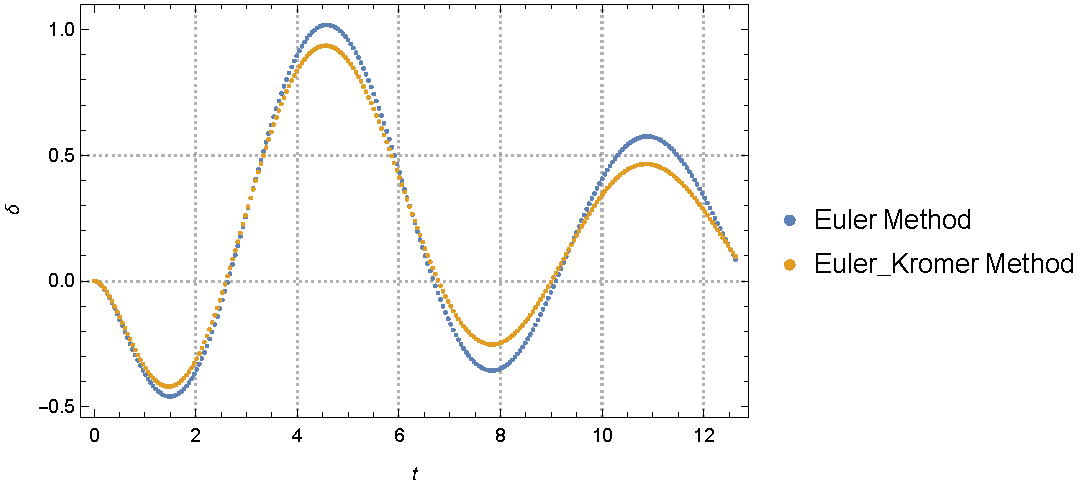
\includegraphics[width=1\linewidth]{plRESer1_250}
  \caption{Погрешность вычисления при $N = 250$.}
  \label{ris:7}
\end{figure}

\subsubsection{Оптимальный выбор метода решения задач на колебательные процессы}
Рассмотрим математический маятник, совершающий малые колебания в поле силы тяжести.
\begin{figure}[h]
  \centering
  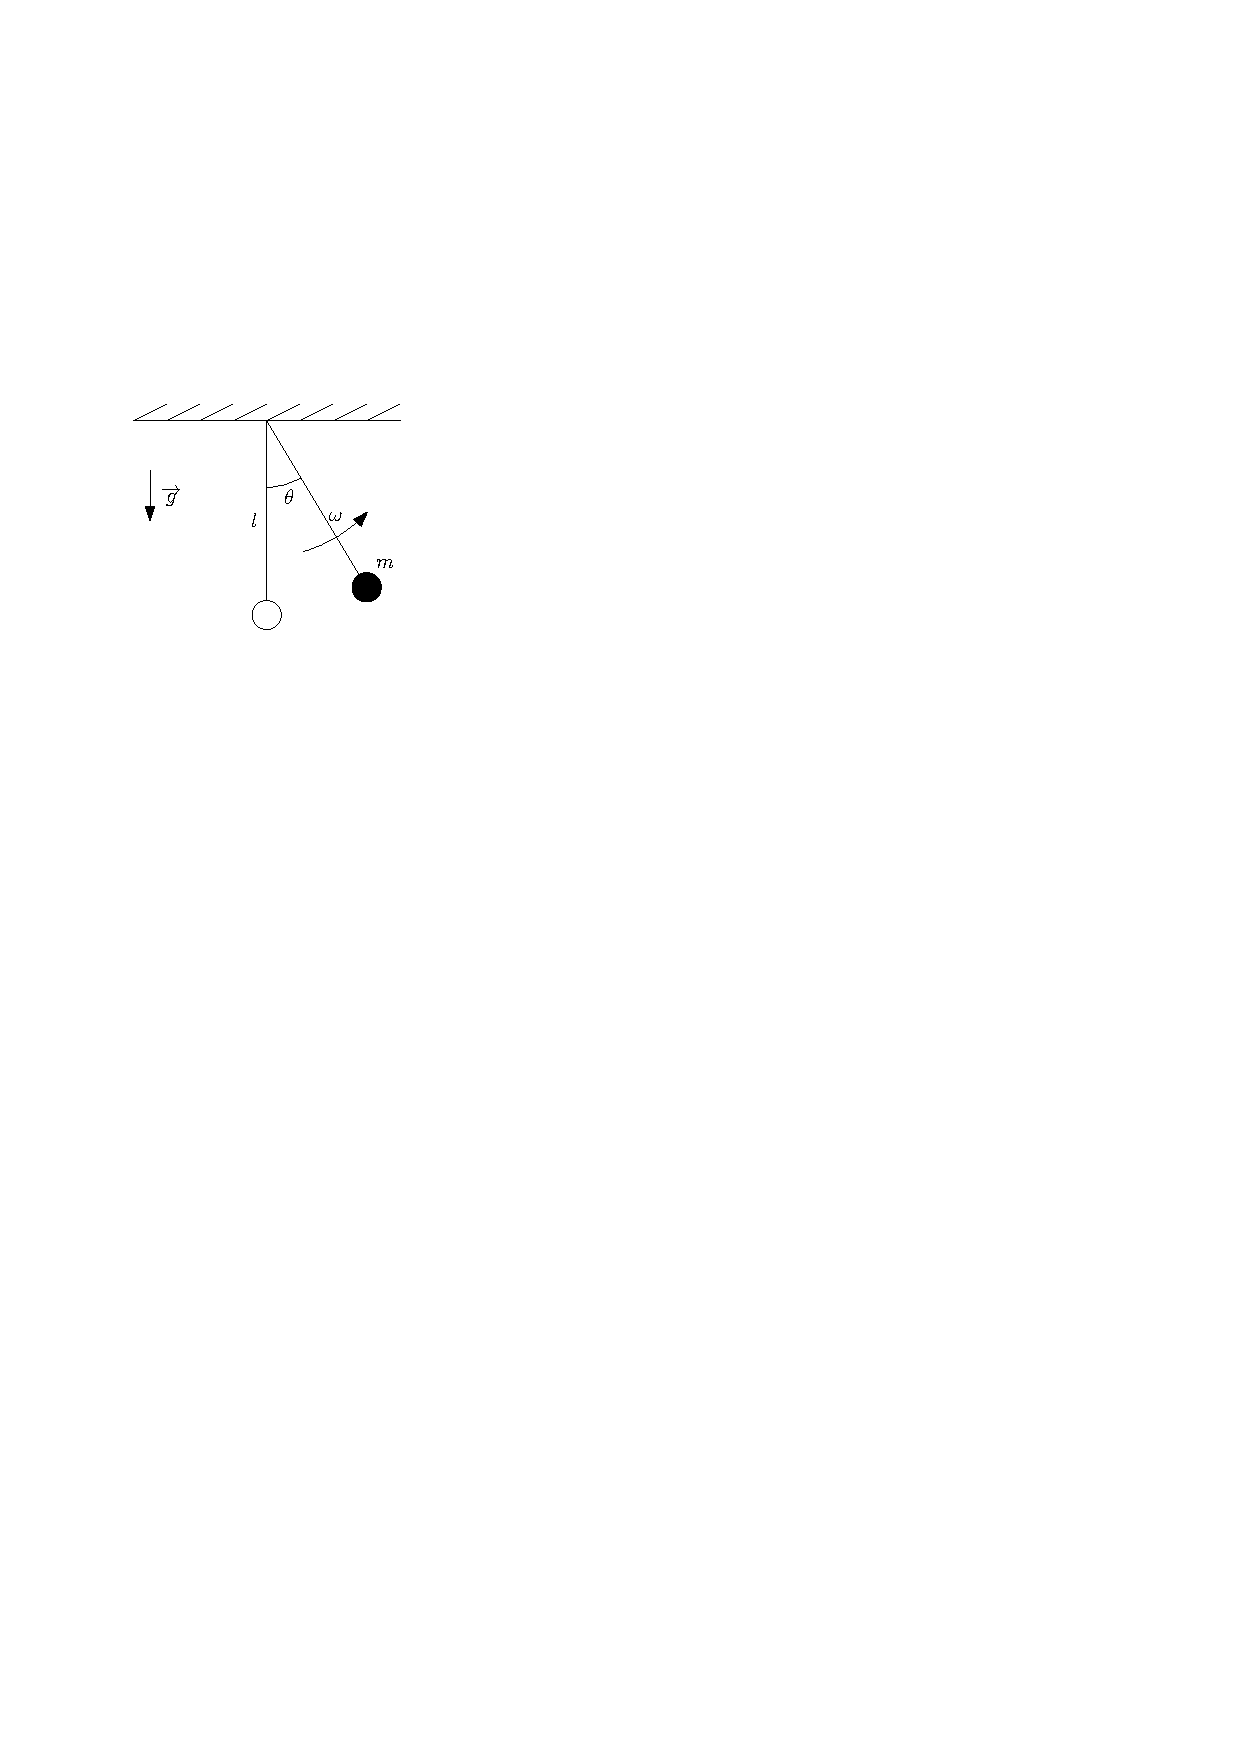
\includegraphics[width=0.3\linewidth]{ris1.pdf}
  \caption{Математический маятник.}
  \label{ris:8}
\end{figure}
Энергия математического маятника: $E = \frac{1}{2} ml^2\omega^2 + mgl(1-\cos(\theta)) \underset{\theta\ll1}\approx \frac{1}{2}ml^2\left(\omega^2 + \frac{g}{l}\theta^2\right)$.\\
Энергия в момент времени $t_{i+1}$:
$$E_{i+1} = \frac{1}{2}ml^2\left(\omega_{i+1}^2 + \frac{g}{l}\theta_{i+1}^2\right).$$
В случае использования метода Эйлера:
\begin{equation}\label{eq22}
\left\{
    \begin{array}{ll}
    \omega_{i+1} = \omega_i - \frac{g}{l}\theta_i\tau,\\
    \theta_{i+1} = \theta_i + \omega_i \tau
  \end{array}
\right.\Rightarrow E_{i+1} = E_i + \frac{mgl}{2}\left(\frac{g}{l}\theta_i^2 + \omega_i^2\right)\tau^2.
\end{equation}
Второе слагаемое выражения (\ref{eq22}) всегда положительно, следовательно, энергия колебаний будет увеличиваться с каждым шагом независимо от его величины.
В случае использования метода Эйлера-Кромера:
$$\left\{
    \begin{array}{ll}
    \omega_{i+1} = \omega_i - \frac{g}{l}\theta_i\tau,\\
    \theta_{i+1} = \theta_i + \omega_{i+1} \tau
  \end{array}
\right.\Rightarrow E_{i+1} = \frac{ml^2}{2}\left[\theta_i^2 + 2\theta_i\left(\omega_i - \frac{g}{l}\theta_i\tau\right)\tau + \left(\omega_i - \frac{g}{l}\theta_i\tau\right)^2\tau^2\right].$$
Пренебрегая величинами более второго порядка малости по $\tau$, получим:
\begin{equation}\label{eq23}
    E_{i+1} = E_i + \frac{g}{l}\left(\omega_i^2 - \frac{g}{l}\theta_i^2\right)\tau^2.
\end{equation}
В уравнение (\ref{eq23}) также как и в (\ref{eq22}) на каждом шаге прибавляется величина порядка $\tau^2$, однако, при ближайшем рассмотрении нетрудно заметить, что первый член в скобках во втором слагаемом в выражении (\ref{eq23}) определяет кинетическую энергию, а второй - потенциальную энергию на данном шаге. При суммировании по всем шагам эти слагаемые сокращаются, следовательно, отсутствует вклад величин второго порядка по $\tau$ и амплитуда колебаний остаётся неизменной на протяжении всего моделирования. Таким образом, выбор метода Эйлера-Кромера более целесообразный при решении ДУ для консервативных колебательных систем.

\newpage
\section{Вывод}
Получено численное решение задачи Коши для ДУ $y' = (2-y) \tan(x)$, $x\in [0,1]$, $y(0) = -1$ стандартным, модифицированным, усовершенствованным методами Эйлера и методом Рунге-Кутта четвёртого порядка. Методами Эйлера и Эйлера-Кромера  численно решена задача об апериодическом колебательном движении: $\ddot{x} + 2 \dot{x} + \frac{x}{4} = 0$, $0<t<3$, $x(0) = 0$, $\dot{x}(0) = 1$, также построены фазовые портреты для точного и численного решений и график погрешности $\delta_n = x(t_n) - x_n$. Результаты получены для $N = 50,\;100,\;250$.

Метод Рунге-Кутта четвёртого порядка показал наибольшую точность при решении ДУ для любого $N$ по сравнению с остальными одношаговыми методами, использованными в данной работе.

Было показано, что метод Эйлера-Кромера имеет большую эффективность, чем метод Эйлера, при рассмотрении консервативных колебательных систем. Также он показал большую точность при решении задачи о свободных затухающих колебаниях.




\end{document} 